\documentclass[unicode,11pt,a4paper,oneside,numbers=endperiod,openany]{scrartcl}

\usepackage{amsmath}
\input{assignment.sty}
\begin{document}


\setassignment
\setduedate{11.11.2020 (midnight)}

\serieheader{High-Performance Computing Lab}{2020}{Student: Gabriele Berra}{Discussed with: - }{Solution for Project 5}{}
\newline

\assignmentpolicy

\section{Task:  Construct adjacency matrices
from connectivity data [10 points]}

With the aim of creating the adjacency matrix from connectivity data, I have divided the problem in  6 sub-tasks as follows:
\begin{enumerate}
	\item Read the \textit{.csv} file;
	\lstinputlisting[frame=single, breaklines=true, tabsize=3, showstringspaces=false, firstline=27 ,lastline=28, language=matlab]{code/read_csv_graphs.m}
	
	\item Initialize a sparse matrix;
	\lstinputlisting[frame=single, breaklines=true, tabsize=3, showstringspaces=false, firstline=45 ,lastline=45, language=matlab]{code/read_csv_graphs.m}

	\item Fill the sparse matrix with 1 if the node $v_i$ is connected with the node $v_j$;
	\lstinputlisting[frame=single, breaklines=true, tabsize=3, showstringspaces=false, firstline=63 ,lastline=65, language=matlab]{code/read_csv_graphs.m}
	
	\item Check the symmetry of the resulting matrix and make it symmetric if it is not;
	\lstinputlisting[frame=single, breaklines=true, tabsize=3, showstringspaces=false, firstline=80 ,lastline=80, language=matlab]{code/read_csv_graphs.m}
	In which the function \textit{symmetry()} is defined as follows:
	\lstinputlisting[frame=single, breaklines=true, tabsize=3, showstringspaces=false, language=matlab]{code/symmetry.m}
	
	\item Visualize the graph;
	\lstinputlisting[frame=single, breaklines=true, tabsize=3, showstringspaces=false, firstline=105 ,lastline=107, language=matlab]{code/read_csv_graphs.m}
	
	\item Save the graph.
	\lstinputlisting[frame=single, breaklines=true, tabsize=3, showstringspaces=false, firstline=114 ,lastline=114, language=matlab]{code/read_csv_graphs.m}
\end{enumerate}

In Fig. \ref{fig:novnEx1} we can see the graph of Norway and Vietnam respectively.

\begin{figure}[h!]
	\centering
	\begin{subfigure}[b]{0.48\textwidth}
	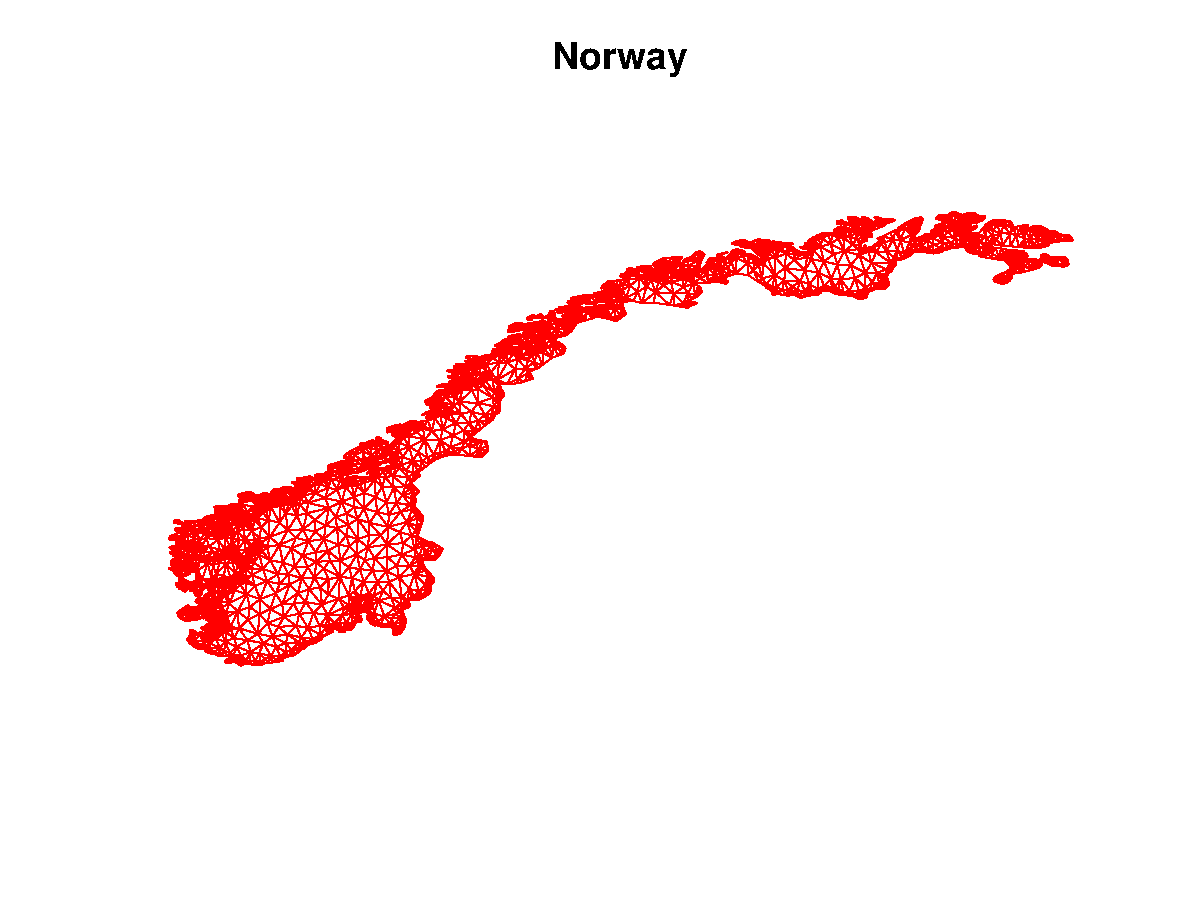
\includegraphics[width=\textwidth]{images/NorwayEx1.eps}
	\end{subfigure}
	\hfill
	\begin{subfigure}[b]{0.48\textwidth}
	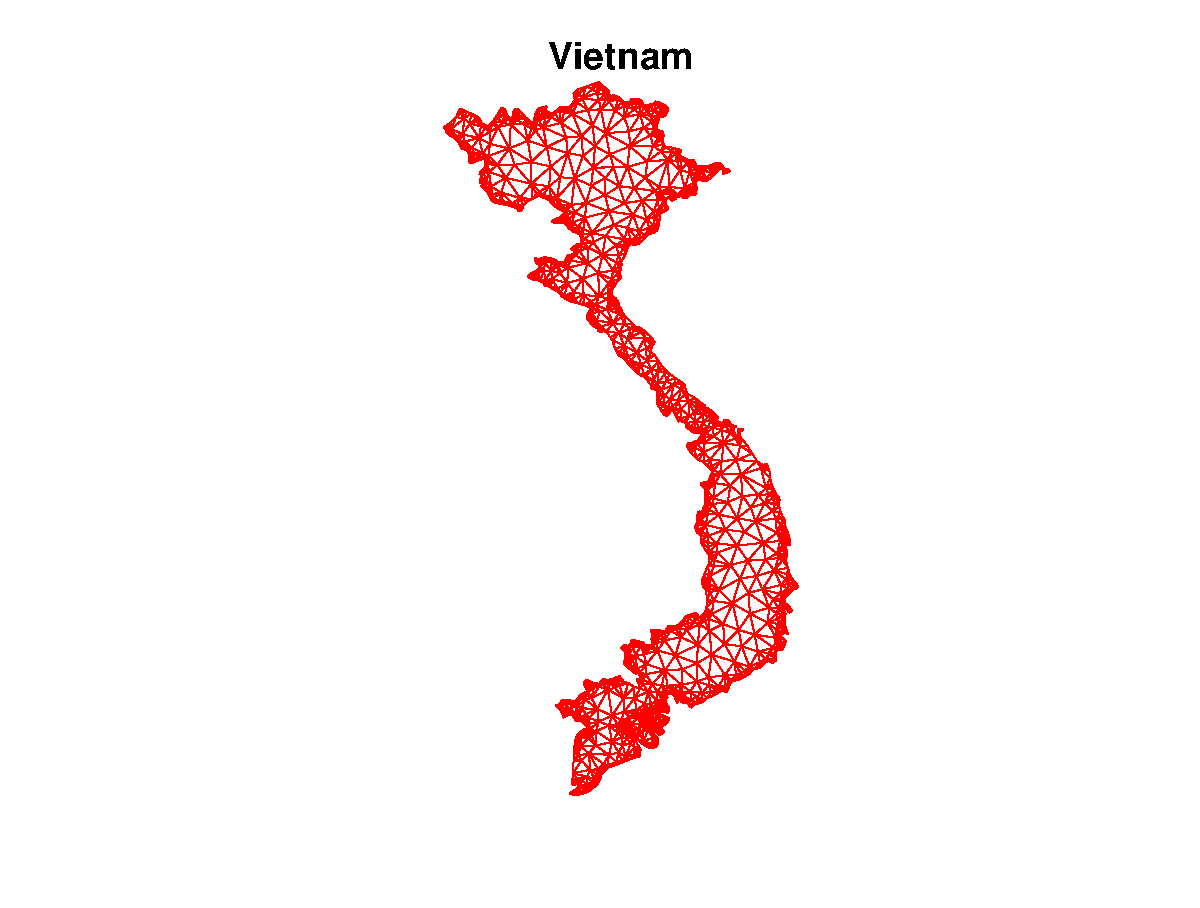
\includegraphics[width=\textwidth]{images/VietnamEx1.eps} 
	\end{subfigure}
	\caption{Left: graph representing Norway. Right: graph representing Vietnam}	
	\label{fig:novnEx1}
\end{figure}


 

\section{Task: Implement various graph partitioning algorithms [30 points]}
\subsection{Spectral Bisection}
In order to perform the spectral bisection, we have to start with the computation of the Laplacian matrix \textbf{L}, which can be assembled from the adjacency matrix \textbf{W} and the degree matrix \textbf{D}. As we know from the theory, matrix \textbf{L} must be a symmetric positive semidefinite matrix in which the smallest eigenvalue is $\lambda_1 = 0$ and the second is $\lambda_2$, with an associated Fiedler's eigenvector $\boldsymbol{\mathbf{v^{(2)}}}$. The next step is to create two partitions - called $V1$ and $V2$ - starting from the Fiedler's eigenvector. The criterion utilised to form the partitions is the following:
\begin{itemize}
	\item If $\boldsymbol{\mathbf{v}}_i^{(2)} < 0, \;\; \boldsymbol{\mathbf{v}}_i^{(2)} \in V1$;
	\item If $\boldsymbol{\mathbf{v}}_i^{(2)} \geq 0, \;\; \boldsymbol{\mathbf{v}}_i^{(2)} \in V2$.
\end{itemize}
Using the function \textit{gplotpart.m}, which takes as input the adjacency matrix, the coordinates, and the first partition ($V1$), I plotted the partitioned graph using spectral bisection. The result is shown in Fig.\ref{fig:spec1e1}.
\begin{figure}[h!]
	\centering
	\includegraphics[width=0.8\textwidth]{images/spectral_mesh1e1.png}
	\caption{Spectral bisection of \textit{mesh1e1.mat}}	
	\label{fig:spec1e1}
\end{figure}


\subsection{Inertial Bisection}
The inertial bisection approach is based on the geometry of the graph. In two dimensions, the algorithm divides the graph by behaving like a "regression-like" method: it searches for the line which minimizes the distance between nodes. 
The first step is to compute the mean of the coordinates $x$ and $y$ as follows:
\begin{equation*}
	\bar x = \frac{1}{n} \sum_{i=1}^n x_i \;\;\; \text{and} \;\;\; \bar y = \frac{1}{n} \sum_{i=1}^n y_i
\end{equation*}
After the computation of the mean value of the coordinates, we can start the creation of matrix \textbf{M}, which contains the sum of the square distances of $x_i$ and $y_i$ from their mean value. Matrix \textbf{M} has the form:
\begin{equation*}
	\boldsymbol{M} = \begin{bmatrix}
		S_{xx} & S_{xy} \\
		S_{xy} & S_{yy}
	\end{bmatrix}
\end{equation*}
Now we can compute the smallest eigenvector and transform it into an orthonormal vector which can be used as input in the function \textit{partition.m}, that gives as output $V1$ and $V2$ (the two partitions). 
An example of partitioned graph is shown in Fig.\ref{fig:inert1e1}.\\\\
\begin{figure}[h!]
	\centering
	\includegraphics[width=0.8\textwidth]{images/inertial_mesh1e1.png}
	\caption{Inertial bisection of \textit{mesh1e1.mat}}	
	\label{fig:inert1e1}
\end{figure}
The results regarding the number of cuts for each mesh and partitioning method are summarized in Table. \ref{table:bisection}.  



\begin{table}[h]
\caption{Bisection results}
\centering
\begin{tabular}{|l|r|r|r|r|} \hline\hline 
Mesh             &  Coordinate           & Metis 5.0.2  & Spectral & Inertial  \\ \hline
mesh1e1          &   18                  &   17         &  17      &  19       \\             
mesh2e1          &   37                  &   37         &  35      &  47       \\ 
netz4504\_dual   &   25                  &   23         &  24      &  30       \\ 
stufe            &   16                  &   16         &  16      &  16       \\
ukerbe1          &   32                  &   27         &  29      &  32       \\
\hline \hline
\end{tabular}
\label{table:bisection}
\end{table}



\section{Task: Recursively bisecting meshes [20 points]}
The implementation has been done according to the description. In Fig.\ref{fig:recbis} we can observe the resulting plot. In Table \ref{table:Rec_bisection} I summarized the results regarding different partitioning methods compared with $p=8$ and $p=16$ for each mesh considered in the exercise.  

\begin{figure}[h!]
	\centering
	\begin{subfigure}[b]{0.45\textwidth}
	\includegraphics[width=\textwidth]{images/spectral_crack.png}
	\caption{Recursive spectral bisection}
	\end{subfigure}
	\hfill
	\begin{subfigure}[b]{0.455\textwidth}
	\includegraphics[width=\textwidth]{images/metis_crack.png}
	\caption{Recursive metis bisection}
	\end{subfigure}
	\vfill
	\begin{subfigure}[b]{0.45\textwidth}
	\includegraphics[width=\textwidth]{images/coordinate_crack.png}
	\caption{Recursive coordinate bisection}
	\end{subfigure}
	\hfill
	\begin{subfigure}[b]{0.455\textwidth}
	\includegraphics[width=\textwidth]{images/inertial_crack.png}
	\caption{Recursive inertial bisection}
	\end{subfigure}
	\caption{Recursive bisection using the function \textit{rec\_bisection.m}}
	\label{fig:recbis}
\end{figure}




\begin{table}[h]
\caption{Edge-cut results for recursive bi-partitioning.}
\centering
\begin{tabular}{|l|r|r|r|r|r|r|r|r|r|} \hline\hline 
\multicolumn{2}{|l|}{Case} & \multicolumn{2}{|r|}{Spectral} & \multicolumn{2}{|r|}{Metis 5.0.2} & \multicolumn{2}{|r|}{Coordinate} & \multicolumn{2}{|r|}{Inertial}    \\ 	
\hline
\multicolumn{2}{|l|}{partitions} & 8 & 16 & 8 & 16 & 8 & 16 & 8 & 16 \\
\hline
\multicolumn{2}{|l|}{mesh3e1} & 75 & 124 & 75 & 117 & 75 & 122 & 76 & 116 \\
\multicolumn{2}{|l|}{airfoil1} & 327 & 578 & 320 & 563 & 516 & 819 & 578 & 903 \\
\multicolumn{2}{|l|}{3elt} & 372 & 671 & 395 & 651 & 733 & 1168 & 880 & 1342 \\
\multicolumn{2}{|l|}{barth4} & 505 & 758 & 405 & 689 & 875 & 1306 & 888 & 1348 \\
\multicolumn{2}{|l|}{crack} & 804 & 1303 & 784 & 1290 & 1343 & 1860 & 1061 & 1618 \\
\hline 
\end{tabular}
\label{table:Rec_bisection}
\end{table}



\section{Task: Comparing recursive bisection to direct $k$-way partitioning [10 points]}
We know from the theory that the recursive bisection method is not as efficient as the k-way method. The former divides the graph in two 'equal' parts, then in four and so on until it reaches the desired number of partitions:  the recursive bisection is - thus - a 'step-by-step' algorithm, in which the $i$-th step depends on the $(i-1)$-th step. If a small error occurs in the first division, it tends to propagate and become bigger in the last cut. In contrast, the $k$-way partitioning method divides directly in $p$ parts the graph and it is, thus, more precise in the majority of the cases. In Fig.\ref{fig:recKway} I reported the partitioned graph of Luxembourg, US, and Russia in which we can notice that - regardless of the country - the $k$-way method performs better than the recursive one. I also summarized the results obtained with the script \textit{Bench\_metis.m} in Table \ref{table:Compare_Metis}.

\begin{figure}[h!]
	\centering
	\begin{subfigure}[b]{0.45\textwidth}
	\includegraphics[width=\textwidth]{images/metis_kway_lux.png}
	\caption{Metis k-way method Lux: 279 cut}
	\end{subfigure}
	\hfill
	\begin{subfigure}[b]{0.45\textwidth}
	\includegraphics[width=\textwidth]{images/metis_rec_lux.png}
	\caption{Metis recursive method Lux: 322 cut}
	\end{subfigure}
	\vfill
	\begin{subfigure}[b]{0.45\textwidth}
	\includegraphics[width=\textwidth]{images/metis_kway_us.png}
	\caption{Metis k-way method US: 961 cut}
	\end{subfigure}
	\hfill
	\begin{subfigure}[b]{0.45\textwidth}
	\includegraphics[width=\textwidth]{images/metis_rec_us.png}
	\caption{Metis recursive method US: 988 cut}
	\end{subfigure}
	\vfill
	\begin{subfigure}[b]{0.45\textwidth}
	\includegraphics[width=\textwidth]{images/metis_kway_russia.png}
	\caption{Metis k-way method Russia: 933 cut}
	\end{subfigure}
	\hfill
	\begin{subfigure}[b]{0.45\textwidth}
	\includegraphics[width=\textwidth]{images/metis_rec_russia.png}
	\caption{Metis recursive method Russia: 1006 cut}
	\end{subfigure}
	\caption{Comparison between $k$-way and recursive partitioning method}
	\label{fig:recKway}
\end{figure}



\begin{table}[h]
\caption{Comparing the number of cut edges for recursive bisection and direct multiway partitioning in Metis 5.0.2.}
\centering
\begin{tabular}{|l|r|r|r|r|r|r|r|r} \hline\hline 
Partitions       &   Luxemburg           & usroads-48 &  Greece &  Switzerland &  Vietnam  &  Norway &  Russia  \\ \hline
 16 (Recursive)  &   197                 & 607        & 297     & 730          & 245       & 284     & 616      \\ 
 32 (Recursive)  &   322                 & 988        & 509     & 1089         & 445       & 470     & 1006     \\        
 16 (k-way)      &   170                 & 607        & 278     & 673          & 245       & 255     & 551      \\
 32 (k-way)      &   279                 & 988        & 471     & 1042         & 411       & 439     & 933      \\ \hline \hline
\end{tabular}              
\label{table:Compare_Metis}
\end{table}



\section{Task: Utilizing graph eigenvectors [30 points]}
In this last section I am going to present the results for this last exercise regarding the usage of eigenvectors.
\begin{enumerate}
	\item [(a)] We know from the theory that the first smaller eigenvector of  matrix \textbf{L} presents the same constant value in every component. The Fiedler's eigenvector has the median in the vicinity of zero and, thus, if we use it for partitioning, we expect to have two vectors of almost the same length (i.e., to obtain to groups that are roughly balanced as far as concerns the number of elements). In Fig.\ref{fig:lambda12} I reported the plot with the first and second eigenvector. 
	\begin{figure}[h!]
		\centering
		\includegraphics[width=0.8\textwidth]{images/eigval12.eps}
		\caption{Plot of the two smallest eigenvectors of the matrix \textbf{L} of the mesh \textit{airfoil1.mat}}
		\label{fig:lambda12}
	\end{figure}
 
	\item [(b)] As asked in the text of the assignment, in Fig.\ref{fig:meshPart} I present the required results.
	
	\begin{figure}[h!]
		\centering
		\begin{subfigure}[b]{0.45\textwidth}
		\includegraphics[width=\textwidth]{images/3elt_3d.png}
		\caption{Partitioning the \textit{3elt} graph}
		\end{subfigure}
		\hfill
		\begin{subfigure}[b]{0.455\textwidth}
		\includegraphics[width=\textwidth]{images/mesh1e1_3d.png}
		\caption{Partitioning the \textit{mesh1e1} graph}
		\end{subfigure}
		\vfill
		\begin{subfigure}[b]{0.45\textwidth}
		\includegraphics[width=\textwidth]{images/barth4_3d.png}
		\caption{Partitioning the \textit{barth4} graph}
		\end{subfigure}
		\hfill
		\begin{subfigure}[b]{0.455\textwidth}
		\includegraphics[width=\textwidth]{images/crack_3d.png}
		\caption{Partitioning the \textit{crack} graph}
		\end{subfigure}
		\caption{Partition of different meshes based on the values of the Fiedler eigenvector}
		\label{fig:meshPart}
	\end{figure}
	
	\item [(c)]	In Fig.\ref{fig:spatspec} I reported the graph of the meshes with the corresponding spectral bi-partitioning using the eigenvectors to supply the coordinates.
	
	\begin{figure}[h!]
		\centering
		\begin{subfigure}[b]{0.45\textwidth}
		\includegraphics[width=\textwidth]{images/3elt_normal.png}
		\caption{Spatial coordinates \textit{3elt}}
		\end{subfigure}
		\hfill
		\begin{subfigure}[b]{0.45\textwidth}
		\includegraphics[width=\textwidth]{images/3elt_strange.png}
		\caption{Spectral coordinates \textit{3elt}}
		\end{subfigure}
		\vfill
		\begin{subfigure}[b]{0.45\textwidth}
		\includegraphics[width=\textwidth]{images/barth4_normal.png}
		\caption{Spatial coordinates \textit{barth4}}
		\end{subfigure}
		\hfill
		\begin{subfigure}[b]{0.45\textwidth}
		\includegraphics[width=\textwidth]{images/barth4_strange.png}
		\caption{Spectral coordinates \textit{barth4}}
		\end{subfigure}
		\vfill
		\begin{subfigure}[b]{0.45\textwidth}
		\includegraphics[width=\textwidth]{images/mesh3e1_normal.png}
		\caption{Spatial coordinates \textit{mesh3e1}}
		\end{subfigure}
		\hfill
		\begin{subfigure}[b]{0.45\textwidth}
		\includegraphics[width=\textwidth]{images/mesh3e1_strange.png}
		\caption{Spectral coordinates \textit{mesh3e1}}
		\end{subfigure}
		\vfill
		\begin{subfigure}[b]{0.45\textwidth}
		\includegraphics[width=\textwidth]{images/crack_normal.png}
		\caption{Spatial coordinates \textit{crack}}
		\end{subfigure}
		\hfill
		\begin{subfigure}[b]{0.45\textwidth}
		\includegraphics[width=\textwidth]{images/crack_strange.png}
		\caption{Spectral coordinates \textit{crack}}
		\end{subfigure}
		\caption{Comparison between plot with spatial coordinates (left) and plot with spectral coordinates (right)}
		\label{fig:spatspec}
	\end{figure}


\end{enumerate}






%\bibliographystyle{plain}
%\bibliography{template}



\end{document}
